%% Document created 28 April 2021 automatically 
%% from /Users/massimosotgia/Desktop/uni_at_DIFI/Lab_C03/setup.py 

%% Copyright (C) Mattia Sotgia et al. 2021
%% Using class lab_unige.cls
%                                                            
%                                                            
%   **                 **             ******   ****   ****   
%  /**                /**            **////** *///** */// *  
%  /**        ******  /**           **    // /*  */*/    /*  
%  /**       ´´´´´´** /******      /**       /* * /*   ***   
%  /**        ******* /**///**     /**       /**  /*  /// *  
%  /**       **´´´´** /**  /** **  //**    **/*   /* *   /*  
%  /********//********/****** /**   //****** / **** / ****   
%  ////////  //////// /////   //     //////   ////   /´///   
%                                                            
%                                                            
\documentclass[italian, a4paper, 10pt, twocolumn]{../../style/lab_unige}
\usepackage[a4paper, margin=1.75cm, footskip=0.25in]{geometry}

\usepackage[utf8]{inputenc}
\usepackage[T1]{fontenc}

\usepackage[italian]{babel}

% \usepackage{biblatex}

\usepackage[bookmarksopen=true, citebordercolor={0 1 0}, linkbordercolor={1 0 0}, urlbordercolor={0 1 1}]{hyperref}
\usepackage[numbered]{bookmark}

\usepackage{graphicx}
\graphicspath{{../fig/}}
\usepackage{array}
\usepackage{tabulary}
\usepackage{booktabs}

% FOUNDAMENTAL
\usepackage{../../style/custom}

\usepackage{physics}

\usepackage{breqn}
\usepackage{cuted}
\usepackage{txfonts}

\usepackage{lipsum}

\usepackage[american]{circuitikz}

%% Define ref types
\newcommand{\reftab}[1]{Tabella {\ref{#1}}}%
\newcommand{\reffig}[1]{Figura {\ref{#1}}}%
\newcommand{\refeqn}[1]{Eq. ({\ref{#1}})}%
\newcommand{\ChiSqr}{$\chi^2$\space}
\newcommand{\ChiNdf}{$\chi^2/\text{ndf}$}
\newcommand{\cernroot}{\texttt{root}}
\newcommand{\treSigma}{$3\sigma$}
\newcommand{\stdErr}[1]{$\varepsilon_{#1}$}
\newcommand{\mstdErr}[1]{\varepsilon_{#1}}
\newcommand{\gLab}{$g_t~=~(~9.8056~\pm~0.0001~\text{ stat}~)~\text{ m/s}^2$}
%% PAPER ONLY custom Macros


%%
\setlength{\columnsep}{6mm}

\begin{document}
    \twocolumn[
    \begin{@twocolumnfalse}
        \title{
            {\raggedright 
\includegraphics[width=0.2\linewidth]{../../style/lab_mark.pdf}\\}
            Metodo Volt-Amperometrico E Circuito RC 
        }
        \author{
        Eugenio Dormicchi\textsuperscript{1, 2},
        % Riccardo Pizzimbone\textsuperscript{1}, 
        Giovanni Oliveri\textsuperscript{1},
        Mattia Sotgia\textsuperscript{1}
        }

        \date{
            \textit{
            \textsuperscript{1}Gruppo C03, Esperienza di laboratorio n. 8 \\
            \textsuperscript{2}In presenza in laboratorio per la presa dati\\
            }
            % Università degli Studi di Genova, Dipartimento di Fisica.\\
            \vspace{2ex}
            (Presa dati
            28 Aprile 2021, 15:00– 18:00; Analisi dati 
            4 Maggio 2021)
        }
        \maketitle
        
        \begin{abstract}
            \textit{Obiettivo-- }
            
            \textit{Metodi-- }
            Circuiti elettrici, carica e scarica condensatori, Fit polinomiali ed esponenziali. 
            \textit{Risultati-- }
        
            \textit{Conclusione-- }
        
        
        \end{abstract}
        \vspace{2em}
    \end{@twocolumnfalse}
    ]

    %%%% CORPO DEL TESTO
    %%%% CORPO DEL TESTO

    \section{Introduzione}
    \label{section:introduction}

    Si vuole misurare il valore delle resistenze $R_1$ e $R_2$ sfruttando il metodo volt-amperometrico, e poi misurare la capacità di un condensatore, a partire dalla misura della costante di tempo su un circuito RC. 

    \subsection{Metodo volt-amperometrico}

    Il metodo volt-amperometrico è un processo sperimentale, che consente di risalire al valore di una resistenza, tramite le misure della tensione ai suoi capi, e dell’intensità di corrente fluente al suo interno. Chiamando $I_R$ la corrente che scorre all’interno della resistenza, e $V_R$ la tensione ai suoi estremi, possiamo calcolare il valore della resistenza $R$, con la formula \[R=\frac{V_R}{I_R}.\]

    Nella prima parte dell’esperienza, misuriamo i valori di due resistenze $R_1$ e $R_2$, mediante il metodo volt-amperometrico. \\
    Il circuito realizzato è composto da un generatore, collegato ad una resistenza nel circuito primario. Sullo stesso circuito è collegato l'amperometro, e in parallelo alla resistenza (posta dopo l'amperometro) è posizionato il voltmetro.
    Il  circuito sul quale sono effettuate le misure è mostrato in \reffig{figure:VI_circ}. 

    \begin{figure}[h!]
        \centering
        \begin{circuitikz} \draw
            (0,4) -- (1,4)
            (1,4) to [ammeter, *-](4,4)
            (4,4) -- (6,4)
            (0,4) to [battery2, l=$V_0$](0,0)
            (0,0) -- (6,0)
            (6,0) to [voltmeter](6,4)
            (4,0) to [R, l=$R$, *-*](4,4)
            ;
        \end{circuitikz}
        \caption{}
        \label{figure:VI_circ}
    \end{figure}
    

    \subsection{Circuito RC}
    
    La seconda parte dell’esperienza si concentrata sullo studio dei processi di carica e scarica di un condensatore in due circuiti RC, in ciascuno dei quali è presente una delle resistenze considerate nella prima parte dell'esperienza. \\
    Il circuito RC è un circuito elettrico semplice, nel quale sono presenti un resistore $R$ e un condensatore $C$ montati in serie; nel circuito è inoltre presente un commutatore posto tra il polo positivo del generatore di tensione e la resistenza $R$. Il commutatore serve per includere ed escludere il generatore dal circuito. Studiando il processo di carica di un condensatore, si può misurare la costante di tempo ($\tau$) del circuito: un valore di tempo indicativo della velocità con la quale avviene il processo di carica.

    La misura della costante di tempo viene effettuata grazie alla variazione di tensioni ai capi della capacità durante la chiusura o l’apertura dell’interruttore.
    La carica del condensatore avviene commutando l’interruttore, al tempo $t_0$, in modo da includere il generatore di corrente nel circuito; la tensione $V_C$ ai capi del condensatore avrà l’andamento seguente
    \begin{equation}
        V_C(t)=V_\infty\left(1-e^{-\frac{t-t_0}{\tau}}\right) \label{equation:carica}
    \end{equation}
    dove $\tau=RC$ è la costante caratteristica di tempo del circuito. Quando il condensatore sarà completamente carico la tensione raggiungerà un valore costante $V_\infty$ che sarà pari a $V_0$ del generatore nel caso ideale in cui il voltmetro ha resistenza interna infinita.

    Successivamente al processo di carica del condensatore spostiamo l’interruttore, scollegando il circuito dal generatore, al tempo $t=0$, affinché il generatore venga escluso dal circuito.
    La tensione VC ai capi del condensatore avrà il seguente andamento
    \begin{equation}
        V_C(t) = V_Ie^{-\frac{t}{\tau}} \label{equation:scarica}
    \end{equation}

    Dove $\tau$ è la stessa costante di tempo del processo di carica e $V_I$ è la tensione ai capi del condensatore  nell’istante in cui viene commutato l’interruttore che quindi sarà inferiore alla tensione di regime.


    % \section{Strumentazione}
    % \label{section:strument}

    \section{Metodi}
    \label{section:methods}

    \subsection{Metodo volt-amperometrico}

    La prima parte dell’esperienza consiste nel misurare due resistenze attraverso il metodo volt-amperometrico. Quest’ultimo rappresenta un modo indiretto di misurazione di resistenze elettriche ed è bastato sulla legge di Ohm.\\
    Il metodo volt amperometrico necessita di un circuito costituito da un generatore di tensione continua che alimenti la resistenza incognita, un amperometro e un voltmetro. Più la resistenza che si intende misurare è piccola più è necessario che la corrente non sia eccessivamente grande per non compromettere la struttura della resistenza e del circuito stesso.

    Esistono due metodi volt-Amperometrici distinti: metodo voltamperometrico con voltmetro a valle e metodo voltamperometrico con voltmetro a monte.\\
    Nella nostra esperienza faremo riferimento alla configurazione con voltmetro posizionato a valle dell’ amperometro \reffig{figure:VI_circ}.\\
    In questa situazione il voltmetro misura la tensione ai capi della resistenza incognita e l’amperometro misura la corrente che circola nella resistenza interna sommata a quella  che permette il funzionamento del voltmetro.\\
    Questo metodo è efficace se la resistenza del voltmetro è molto maggiore della resistenza incognita poiché la resistenza equivalente di due resistenze poste in parallelo è $R_{eq}=(R_V R)/(R_V+R)$ (dove $R$ è la resistenza incognita e $R_V$ è quella del voltmetro).
    Considerando trascurabili gli effetti dovute alle resistenza interne degli strumenti, si ottiene $I_A$ circa $I_R$ e $V_V$ circa $V_R$. 
    Variando la tensione $V_0$ del generatore è possibile misurare coppie di valori $V_V$ e $I_A$.  I valori misurati sono legati dalla relazione lineare \begin{equation}
        V_V =RI_A \label{equation:VI}
    \end{equation} di conseguenza è possibile ottenere $R$ incognita.

    Il circuito sulla basetta è stato già predisposto dai docenti, il nostro primo scopo è collegare in modo corretto il circuito al generatore, al  multimetro da banco e al Tester.
    Per la prima parte è necessario che il multimetro da banco sia impostato in modalità di lettura di correnti continue (tasto DC) mentre il tester sia impostato in modalità di lettura di tensioni continue.\\
    Utilizziamo l’Output-1 del generatore collegando l’uscita positiva di quest’ultimo  all’amperometro nella boccola dei milliAmpere attraverso un cavo schermato. Un secondo cavo uscente dal foro comune dell’amperometro viene mandato ai capi della resistenza cioè al terminale giallo andando così a costituire la corrente entrante; infine colleghiamo l’ingresso nero con un terzo filo (di diverso colore per distinguerlo dai precedenti) all’uscita negativa del generatore, chiudendo così il circuito.

    Successivamente colleghiamo il nostro tester, che svolgerà la funzione di voltmetro, in parallelo alla resistenza.\\
    Esso dispone di un foro centrale, che costituisce l’uscita comune, e a destra di quest’ultimo un secondo foro per le tensioni continue. Colleghiamo quindi l’uscita delle tensioni del tester dietro al cavo dell’amperometro (boccola gialla) mentre il cavo di ritorno nero dietro la boccola nera fino all'entrata comune (COM) del tester.\\
    Per sicurezza si può utilizzare il comando Display Limit così di limitare la potenza erogata dal generatore e non danneggiare il circuito.

    Per ciascuna delle due resistenze eseguiamo i seguenti passaggi: inizialmente montiamo la resistenza incognita  all’ interno del circuito facendo attenzione che il generatore non stia erogando tensione. Successivamente effettuiamo 6  coppie misure di $V_V$ e $I_A$ variando la tensione $V_0$ erogata dal generatore in un intervallo da 0~V fino a 10~V.  

    Tutte le misure vanno fatte utilizzando il fondo scala più appropriato per ciascuno strumento e della misura che si effettua; ci segnamo di volta in volta il fondo scala utilizzato: questo permetterà di associare ai valori le relative incertezze deducibili dai data sheet. Infine eseguiamo un fit lineare e ricaviamo il valore delle due resistenze $R_1$ e $R_2$.

    \subsection{Circuito RC}

    Inizialmente il nostro compito è collegare correttamente il circuito al multimetro da banco, impostato in modalità di lettura di tensioni continue, e al generatore di corrente.\\
    Congiungiamo il circuito al generatore: l’uscita negativa di quest’ultimo viene collegata alla boccola nera mentre quella positiva viene collegata al terminale rosso della basetta.\\
    Successivamente scolleghiamo il tester e andiamo a collegare il multimetro da banco che svolgerà la funzione di voltmetro.

    Colleghiamo attraverso un cavo l’uscita COM del multimetro alla boccola nera della basetta mentre con un secondo cavo attacchiamo l’uscita della tensione positiva all’ingresso verde. Prima di procedere alla presa dati è importante verificare che il multimetro sia impostato correttamente in lettura di tensioni continue, selezionando il tasto DCV; inoltre è necessario selezionare il fondo scala dei 2~Volt e impostarlo in \verb|manual range|. Infine montiamo la resistenza misurata in precedenza posizionandola nei fori corretti sulla basetta.

    Dopo aver verificato che il tutto sia montato correttamente si può procedere con la seconda parte dell’ esperienza.

    Questa consiste nell’ utilizzo delle due resistenze misurate precedentemente all’ interno del circuito descritto sopra di cui dobbiamo trovare la constante di tempo nel processo di carica e scarica.

    La misura viene effettuata attraverso il programma DMMDaq che acquisisce a intervalli di tempo costanti la tensione letta dal multimetro da banco. Per ciascuna misura è necessario acquisire dati per una durata pari a circa 2-3 costanti di tempo da quando l’interruttore viene commutato.  Scegliamo infine una frequenza di acquisizione appropriata in modo da ottenere circa 5-10 misure per ogni costante di tempo. 

    Procediamo quindi con la misura di carica: impostiamo la tensione del generatore ad un valore compreso tra i 0.2~V e i 2~V che verrà mantenuta costante durante la misura; nel nostro caso abbiamo selezionato una tensione costante erogata dal generatore $1$~V.\\
    Commutiamo l’interruttore in modo da escludere il generatore e attendiamo sufficientemente a lungo finché la tensione letta dal multimetro  sia compatibile con zero. 

    Successivamente facciamo partire il programma dal terminale e gli forniamo i comandi seguenti: \verb|T|, \verb|t|, nome del file in cui salvare i dati e intervallo di tempo di acquisizione $\Delta t$. 

    Per la prima resistenza è conveniente scegliere un $\Delta t$ di 0.5~s mentre per la seconda un intervallo di 1~s. Appena dopo aver fatto partire l’ acquisizione spostiamo l'interruttore così da includere il generatore e interrompiamo la presa dati dopo circa 2-3 costanti di tempo del circuito (45 secondi per la prima resistenza e 90 secondi per la seconda, stimando come costanti di tempo $\tau_1\approx$10~s e $\tau_2\approx$30~s).

    Completata la misura di carica procediamo con quella di scarica mantenendo sempre il circuito in tensione:  prepariamo il programma di acquisizione dati inserendo gli stessi comandi dati in precedenza e lo stesso intervallo di tempo tra due misure successive usato per il processo di carica. \\
    Commutiamo l’ interruttore escludendo il generatore e immediatamente dopo facciamo partire  l’acquisizione dati. Analogamente a prima interrompiamo il programma dopo un tempo circa pari a 2-3~$\tau$.
    Dopo aver concluso le misure di carica e scarica del circuito RC utilizzando la resistenza $R_1$, procediamo con la resistenza $R_2$ ripetendo i medesimi passaggi.

    Come controllo finale è possibile misurare direttamente le resistenze impostando il multimetro in modalità ohmmetro. \\
    Scolleghiamo quindi le parti del circuito non essenziali, collegando infine la boccola nera all’ uscita comune del multimetro e la boccola rossa al foro di lettura delle resistenze. I valori forniti dal multimetro dovranno essere poi confrontati con quelli ottenuti attraverso il metodo volt-amperometrico.


    \section{Analisi dati}
    \label{section:analysis}

    \subsection{Stima delle resistenze}

    \begin{figure}
        \centering
        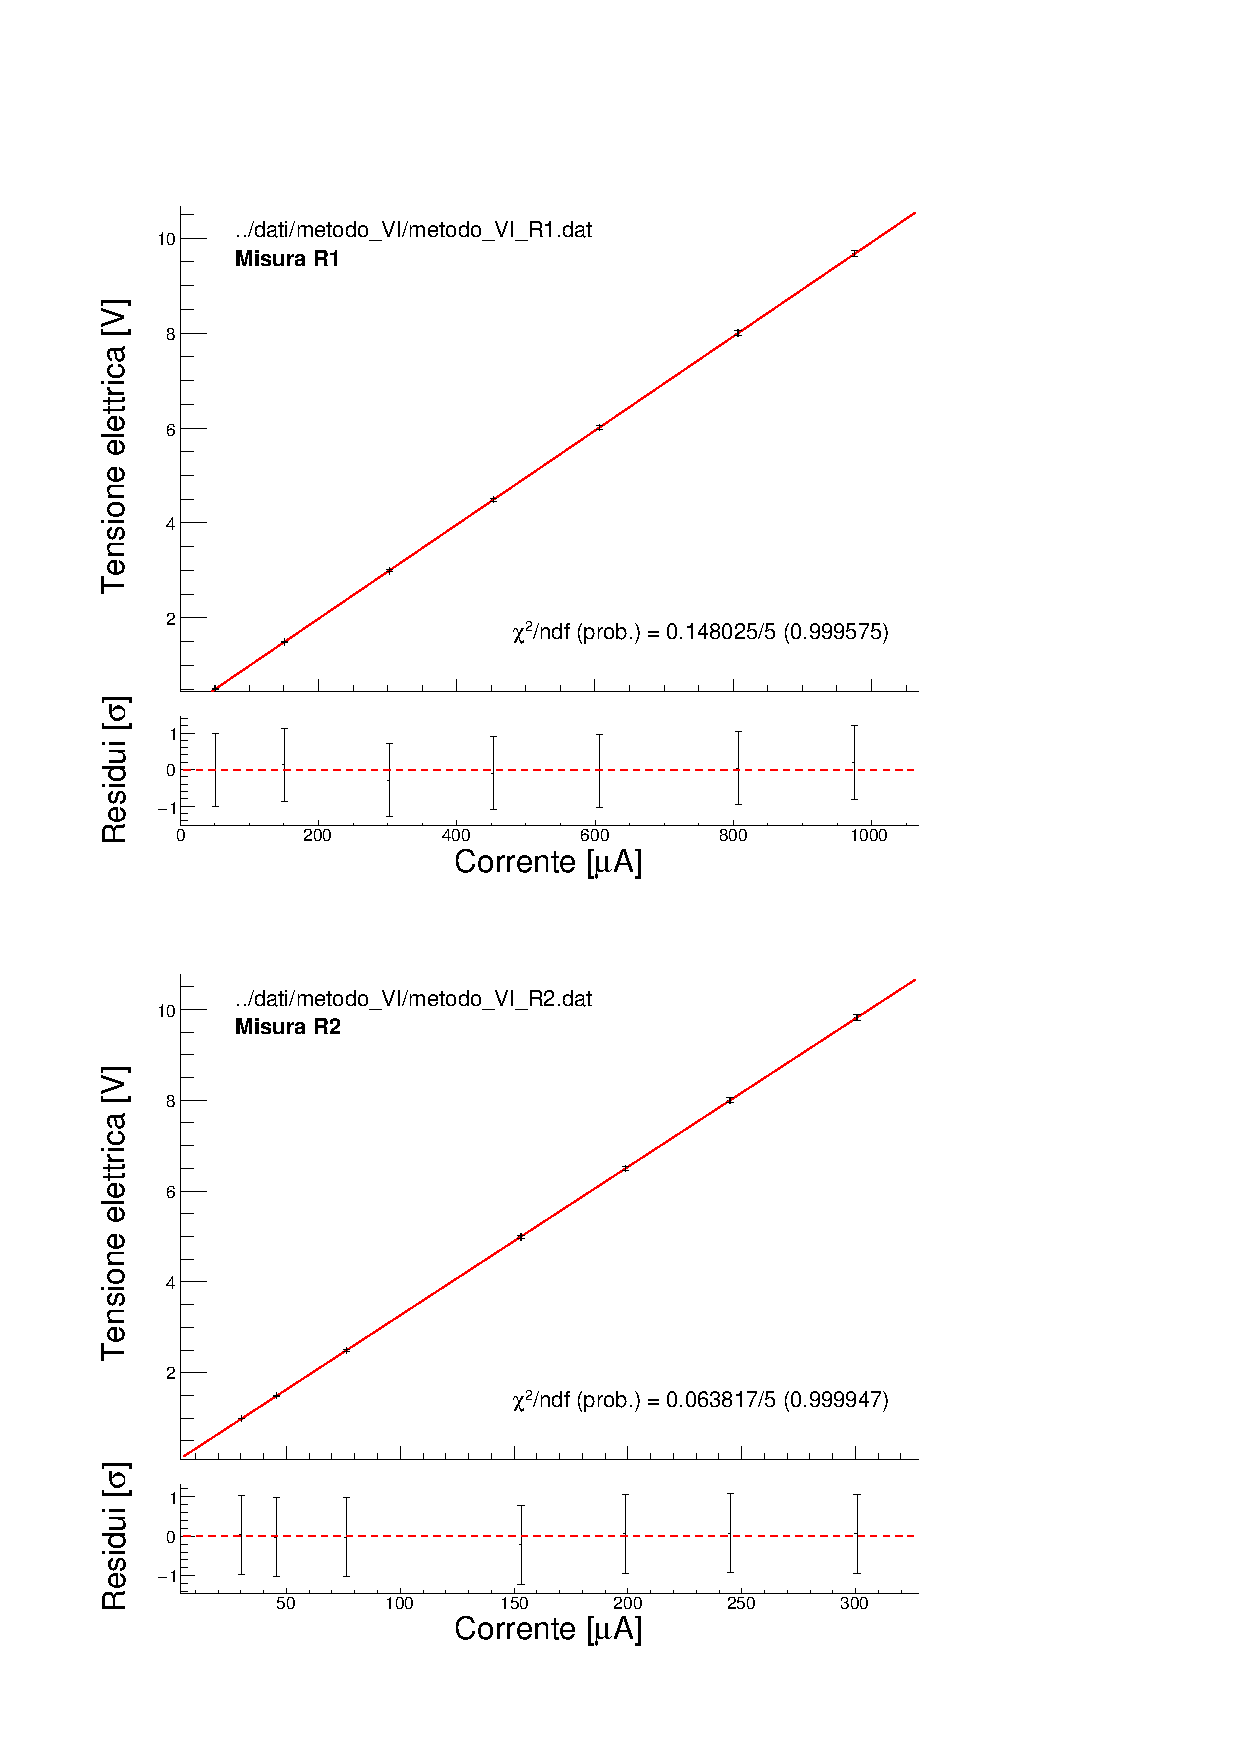
\includegraphics[width=\linewidth]{misura_R1_R2.pdf}
        \caption{}
        \label{figure:plot_R1_R2}
    \end{figure}

    Rappresentiamo le coppie ($I_A$, $V_V$) trascritte in TABELLA nella \reffig{figure:plot_R1_R2}, dove possiamo osservare un andamento lineare. Per le coppie ($I_A$, $V_V$) consideriamo come incertezza il valore deducibile dal data-sheet.\\
    Per la corrente $I_A$ l'errore 
    \[
        \mstdErr{I_A} = \left \{
            \begin{aligned}
                0.03\%\cdot\text{valore}+0.05\%\cdot\text{range  (se range}=200~\mu\text{A)}\\
                0.02\%\cdot\text{valore}+0.05\%\cdot\text{range  (se range}=2~\text{mA)}
            \end{aligned}
            \right .
    \]
    mentre per la tensione il valore è
    \[
        \mstdErr{V_V} = \left \{
            \begin{aligned}
                0.015\%\cdot\text{valore}+0.001 \text{  (se range}=2~V)\\
                0.015\%\cdot\text{valore}+0.01 \text{  (se range}=20~V)
            \end{aligned}
            \right .
    \]
    dove \textit{range} indica il fondoscala scelto.

    Dalla \refeqn{equation:VI} possiamo ricavare una relazione lineare rappresentabile da una polinomiale di primo grado (\verb|pol1| in \cernroot) come $a_0 + a_1x = y$, dove $a_0$ deve essere compatibile con 0.\\
    Dal Fit possiamo ricavare una stima di $R_1$ e $R_2$. In \reffig{equation:VI} rappresentiamo anche i grafici dei residui, dove il valore sulle $x$ è lo stesso, mentre sulle $y$ poniamo
    \[
        \frac{V_{\text{misurata}}-V_{fit}}{\mstdErr{V_{\text{misurata}}}}.
    \]
    che rappresenta lo spostamento del valore misurato dal Fit, normalizzato, a cui è associato un errore pari a $1\sigma$. In questa considerazione stiamo assumendo che la distribuzione di probabilità dei singoli punti sia Gaussiana.

    \subsection{Stima delle costanti di tempo}

    Dai file raccolti dal software DMMDaq riportati nell'appendice \ref{section:appendix_EXT_DATA} rappresentiamo in \reffig{figure:plot_RC} le coppie ($t$, $V_C(t)$) per i processi di carica e scarica relativi alle due resistenze. \\
    L'errore relativo a $t$ si assume essere $\mstdErr{t}=0.005\cdot T$ dove $T=\Delta t$ è l'intervallo che intercorre tra due misurazioni. Per l'errore relativo a $V_C$ consideriamo la maggiore tra le seguenti quantità: 
    \[
        \mstdErr{V_C} = \frac{1}{\sqrt{12}}\left|V_{(i)}-V_{(i-1)}\right|\frac{0.3~\text{s}}{T}  
    \]oppure l'incertezza deducibile dal data-sheet dello strumento.


    \begin{figure*}
        \centering
        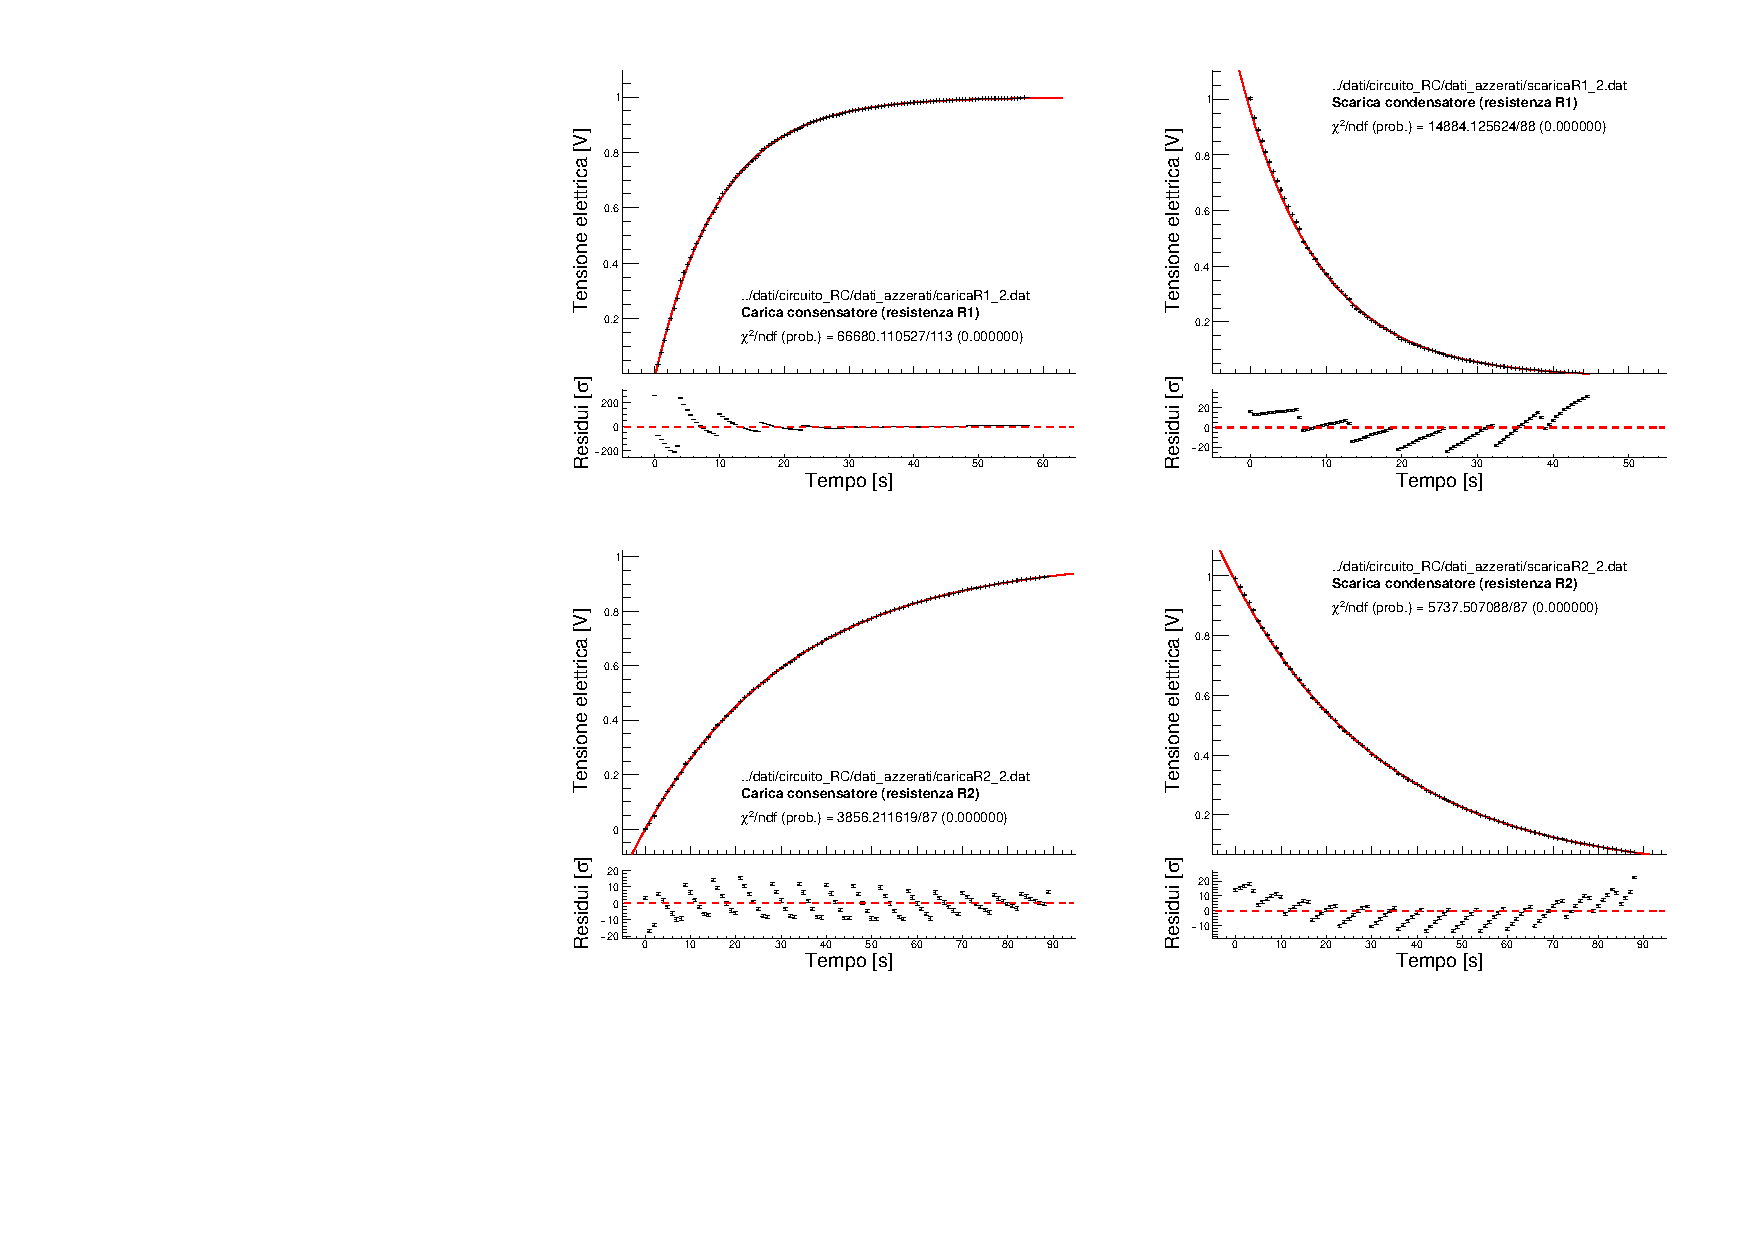
\includegraphics[width=\linewidth]{plot_RC.pdf}
        \caption{}
        \label{figure:plot_RC}
    \end{figure*}

    \section{Risultati}
    \label{section:results}

    \section{Conclusione}
    \label{section:conclusion}

    \subsection{Controlli}

    \subsection{Possibili errori sistematici}

    \appendix

    \setcounter{table}{0}
    \renewcommand{\thetable}{A\arabic{table}}

    \section{Dati estesi}
    \label{section:appendix_EXT_DATA}
    

\end{document}
    
